\label{chapter_1}
%
\vskip-.1cm
\epigraph{``I have of late, (but wherefore I know not) lost all my mirth, forgone all custom of exercises; and indeed, it goes so heavily with my disposition; that this goodly frame the earth, seems to me a sterile promontory; this most excellent canopy the air, look you, this brave o'er hanging firmament, this majestical roof, fretted with golden fire: why, it appeareth no other thing to me, than a foul and pestilent congregation of vapours. What a piece of work is man, How noble in reason, how infinite in faculty, In form and moving how express and admirable, In action how like an Angel, In apprehension how like a god, The beauty of the world, The paragon of animals.''}{Hamlet\cite{Schottdorf2013}, 1601}
%
\vskip-.1cm
\section{Content}
\lipsum[1-1]
%
%
\newpage
\section{Introduction}
Every scientific text needs a good introduction.
\lipsum
%
%
%
\section{Results}
In the results, there are tables, for instance \ref{tab_1}, and figures, for instance \ref{fig1}.
%
\begin{table}
\begin{center}
\begin{tabular}{l c c c c} \hline
$\epsilon\,[\text{deg}]$  & $k_\text{pref}\,[\text{cyc}/\text{deg}]$ & $M[\text{mm}_c/\text{deg}]$ & $k_\text{pref}\,[\text{cyc}/\text{mm}_c]$ & $\lambda\,[\text{mm}_c$] \\
\hline
\rowcolor{gray!50}0 - 5     & 1.3 & 1.2 & 1.1 & 0.9 \\
5 - 10    & 0.6 & 0.5 & 1.2 & 0.8 \\
\rowcolor{gray!50} 23 [m623] & 0.7 & 0.4 & 1.8 & 0.6 \\ \hline
\end{tabular}
\caption{A good chaption}
\label{tab_1}
\end{center}
\end{table}
%
\lipsum
%
\begin{figure}
\centering
 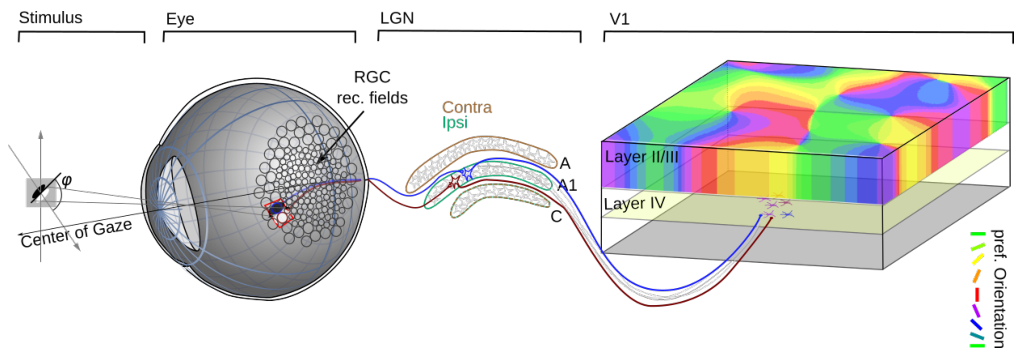
\includegraphics[width=\linewidth]{./chapter_1/fig1/fig1.pdf}
\caption{\label{fig1} \textbf{A nice figure.} \textbf{A} Try to use vector files. I recomment inkscape.}
\end{figure}




